\section{Experiments}

\begin{table*}[!ht]
    \centering
    % \setlength\tabcolsep{2.9pt}
 % \renewcommand{\arraystretch}{0.9}
 \caption{Performance comparison across different methods. RePR $\uparrow$: reliable pass rate. Tool Hallu $\downarrow$: tool hallucination rate. Tool Num $\downarrow$: average tool calling number. Utility: Benifit-cost utility$\downarrow$.}
 \begin{adjustbox}{width=0.98\textwidth}
    \begin{tabular}{lcccccccccccccccc}
        \toprule
        \multirow{4}{*}{\textbf{Method}} & \multicolumn{4}{c}{\thead{I1 Instruction \\ Solvable + Unsolvable}} & \multicolumn{4}{c}{\thead{I2 Category \\ Solvable + Unsolvable} }& \multicolumn{4}{c}{\thead{I3 Instruction \\ Solvable + Unsolvable}}& \multicolumn{4}{c}{Overall} \\
        \cmidrule(rl){2-5} \cmidrule(rl){6-9} \cmidrule(rl){10-13} \cmidrule(rl){14-17}
        & RePR$\uparrow$ & \thead{Tool \\ Hallu}$\downarrow$ & \thead{Tool \\ Num}$\downarrow$ & Utility$\uparrow$ & RePR$\uparrow$ & \thead{Tool \\ Hallu}$\downarrow$ & \thead{Tool \\ Num}$\downarrow$ & Utility$\uparrow$ & RePR$\uparrow$ & \thead{Tool \\ Hallu}$\downarrow$ & \thead{Tool \\ Num}$\downarrow$ & Utility$\uparrow$ & RePR$\uparrow$ & \thead{Tool \\ Hallu}$\downarrow$ & \thead{Tool \\ Num}$\downarrow$& Utility$\uparrow$ \\
        \midrule
    \rowcolor{gray!8}\multicolumn{17}{c}{\textit{Closed-source LLMs}}\\
     \midrule
     \texttt{gpt-3.5-turbo}  & 66.9 & 57.0 & 5.6 & 8.0 & 57.6 & 64.4 & 7.3 & 4.9 & 50.7 & 68.9 & 11.0 & 2.6 & 58.4 & 63.4 & 8.0 & 5.2 \\
     \texttt{GPT 4o-mini}  & 77.2 & 11.4 & 1.7 & 13.6 & 74.9 & 19.2 & 2.0 & 12.8 & 67.7 & 23.2 & 3.3 & 10.2 & 73.3 & 17.9 & 2.3 & 12.2 \\
     \texttt{GPT 4o}   & 80.1 & 5.9 & 1.2 & 14.8 & 75.1 & 9.6 & 1.3 & 13.3 & 69.1 & 9.5 & 1.8 & 11.9 & 74.8 & 8.3 & 1.4 & 13.4\\
        \midrule
        \rowcolor{gray!8}\multicolumn{17}{c}{\textit{Toolllama (7B)}~\citep{qin2023toolllm}}\\
        \midrule
        \texttt{Baseline} & 64.2 & 55.1 & 3.3 & 8.8 & 64.4 & 56.4 & 3.7 & 8.4 & 58.9 & 57.9 & 4.1 & 6.9 & 62.5 & 56.5 & 3.7 & 8.0 \\
        \texttt{\ \ \  + RLHF}  & 65.1 & 54.2 & 3.2 & 9.0 & 64.6 & 55.7 & 3.5 & 8.7 & 58.5 & 57.5 & 4.1 & 6.7 & 62.7 & 55.8 & 3.6 & 8.1 \\
         \texttt{\ \ \  + Steptool} &67.2 & 53.7 & 3.3 & 10.2 &
         66.8 & 55.9 & 3.7 & 9.4 &
         56.7 & 59.0 & 4.3 &6.2 & 63.6 & 56.2 & 3.8 & 8.6
         \\
         \hdashline
        \texttt{\ \ \  +  SFT}   & 67.8 & 24.8 & 2.1 & 10.8 & 67.6 & 32.7 & 2.6 & 10.3 & 65.7 & 29.6 & 2.5 & 9.9 & 67.0 & 29.0 & 2.4 & 10.3 \\
        \texttt{\ \ \  +  DPO}  & 66.1 & 41.5 & 1.2 & 11.2 & 66.9 & 35.7 & 1.2 & 11.4 & 63.5 & 46.0 & 1.3 & 10.3 & 65.5 & 41.1 & 1.2 & 11.0   \\
        \texttt{\ \ \  +  SFT\&DPO}  & \textbf{71.4} & 25.8 & 2.1 & 11.8 & \textbf{69.0} & 32.4 & 2.5 & 10.9 & 66.6 & 32.1 & 2.5 & 9.9 & 69.0 & 30.1 & 2.4 & 10.9 \\
        \texttt{\ \ \  + Relign}  & 68.2 & \textbf{17.1} & \textbf{0.9} & \textbf{12.2} & 68.3 & \textbf{21.6} & \textbf{0.9} & \textbf{12.2} & \textbf{71.0} & \textbf{16.3} & \textbf{1.0} & \textbf{13.0} & \textbf{69.1} & 1\textbf{8.3} & \textbf{0.9} & \textbf{12.4}   \\
        \midrule
        \rowcolor{gray!8}\multicolumn{17}{c}{\textit{Llama3.1 (8B)}~\citep{dubey2024llama}}\\
        \midrule
        \texttt{Baseline}     & 68.5 & 51.2 & 2.1 & 10.5 & 66.1 & 51.7 & 2.3 & 9.4 & 61.3 & 49.6 & 2.4 & 8.3 & 65.3 & 50.8 & 2.2 & 9.4 \\
        \texttt{\ \ \  + RLHF}     & 68.5 & 51.7 & 2.4 & 10.2 & 66.5 & 50.8 & 2.6 & 9.4 & 61.0 & 49.1 & 2.7 & 7.9 & 65.3 & 50.5 & 2.6 & 9.2 \\
        \texttt{\ \ \  + Steptool}    & 71.1 & 50.8 & 2.0 & 11.2 & 69.7 & 52.0 & 2.3 & 10.5 & 56.3 & 55.8 & 2.5 & 6.8 & 65.7 & 52.9 & 2.3 & 9.5 \\
        \hdashline
        \texttt{\ \ \  +  SFT}  & 71.6 & 17.3 & 1.4 & 12.1 & 71.3 & 24.2 & 1.7 & 11.8 & 66.0 & 28.6 & 2.1 & 9.7 & 69.6 & 23.4 & 1.7 & 11.2 \\
        \texttt{\ \ \  +  DPO} & 69.6 & 43.3 & 2.0 & 11.8 & 67.2 & 44.9 & 2.2 & 11.1 & 62.2 & 50.2 & 2.7 & 9.0 & 66.3 & 46.1 & 2.3 & 10.6   \\
        \texttt{\ \ \  +  SFT\&DPO}  & 77.2 & 14.0 & 1.4 & 13.5 & 72.5 & \textbf{19.0} & 1.6 & 11.5 & 71.5 & 20.1 & 2.0 & 10.9 & 73.7 & 17.7 & 1.7 & 12.0 \\
        \texttt{\ \ \  +  Relign }     & \textbf{80.5} & \textbf{8.7} & \textbf{1.3} & \textbf{14.5} & \textbf{75.8} & 22.1 & \textbf{1.6} & \textbf{12.5} & \textbf{75.3} & \textbf{13.1} & \textbf{1.8} & \textbf{12.4} & \textbf{77.2} & \textbf{14.6} & \textbf{1.5} & \textbf{13.2} \\
        \midrule
        \rowcolor{gray!8}\multicolumn{17}{c}{\textit{Qwen2.5 (7B)}~\citep{yang2024qwen2}}\\
        \midrule
        \texttt{Baseline}    & 71.5 & 46.1 & 2.2 & 10.9 & 66.2 & 49.6 & 2.4 & 9.4 & 57.7 & 51.9 & 2.7 & 6.8 & 65.1 & 49.2 & 2.4 & 9.1 \\
        \texttt{\ \ \  + RLHF}  & 67.8 & 48.7 & 2.3 & 10.7 & 65.4 & 47.3 & 2.4 & 9.8 & 62.8 & 49.4 & 2.6 & 9.6 & 65.3 & 48.5 & 2.5 & 10.0  \\
        \texttt{\ \ \  + Steptool}   & 69.5 & 46.8 & 2.4 & 10.2 & 69.6 & 46.6 & 2.5 & 10.2 & 62.7 & 46.0 & 2.8 & 8.0 & 67.3 & 46.5 & 2.6 & 9.5 \\
         \hdashline
        \texttt{\ \ \  +  SFT} & 69.9 & 18.7 & 1.5 & 11.6 & 69.9 & 25.2 & 1.7 & 11.4 & 62.7 & 33.1 & 2.0 & 8.8 & 67.5 & 25.7 & 1.7 & 10.6  \\
        \texttt{\ \ \  +  DPO}  & 69.9 & 45.0 & 2.3 & 10.6 & 68.7 & 45.5 & 2.4 & 10.0 & 65.2 & 45.9 & 2.9 & 8.7 & 67.9 & 45.4 & 2.5 & 9.8   \\
        \texttt{\ \ \  +  SFT\&DPO}   & 69.8 & 20.6 & 1.5 & 11.4 & 69.7 & 25.8 & 1.7 & \textbf{11.3} & 58.8 & 27.6 & 2.0 & 8.0 & 66.1 & 24.7 & 1.7 & 10.2 \\
        \texttt{\ \ \  + Relign} & \textbf{77.0} & \textbf{12.0} & \textbf{1.3} & \textbf{13.3} & \textbf{69.0} & \textbf{22.6} & \textbf{1.7} & 10.6 & \textbf{72.9} & \textbf{18.3} & \textbf{2.0} & \textbf{11.6} & \textbf{73.0} & \textbf{17.6} & \textbf{1.7} & \textbf{11.9}  \\
        \bottomrule
    \end{tabular}%
    \end{adjustbox}
\label{table:main_res}
\end{table*}
% \input{tables/benifit_cost_ratio.tex}


\subsection{Experimental Setup}

\paragraph{Datasets.} In our experiments, we primarily utilized three datasets:  \textbf{ToolBench}, \textbf{StableToolBench} and \textbf{RelyToolBench}. ToolBench~\cite{qin2023toolllm} was constructed by scraping various APIs from RapidAPI and generating corresponding tasks and executions, comprising a total of 120,000 data samples. StableToolBench~\cite{guo2024stabletoolbench} is a selected subset of solvable samples from ToolBench, and it also proposed a stable environment for evaluation.  We randomly select 10,000 samples from Toolbench for constructing reliability alignment data. We further construct RelyToolBench based on StableToolBench for evalution.

% ToolBench is utilized for training purposes, from which we extracted 10,000 samples to construct our Reliable Alignment training dataset. In addition to these samples, we also randomly sampled a portion of the data to introduce additional tool replacements and construct missing parameters, similar to the evaluation of StableToolBench.

\paragraph{Baselines.} (1) \textbf{RLHF \& StepTool.}  The two baselines are proposed in Steptool~\cite{yu2024steptool}, which augments tool learning by introducing step-level rewards. RLHF is a simplified reinforcement learning version of Steptool with only trajectory-level reward. (2) \textbf{SFT \& DPO.} We also implemented a joint training approach that combines SFT and DPO losses on the same base model as baseline. The combination ratio is set to 0.5.


%SFT learns from correct tool-call traces, while DPO ranks trajectories based on hallucination severity. Their combination enhances tool-use stability and reduces invalid calls. %我们实现了基于同一个基座模型，同时使用DPO和SFT的loss进行混合训练

% \paragraph{Relign.}  
% Relign expands the action space, allowing deferrals and corrections to mitigate hallucinations. It integrates preference optimization and structured training to improve reliability and efficiency.


\paragraph{Training and inference details.}
We use \textsc{Llama-3.1-8B-Instruct}, \textsc{Qwen-2.5-7B-Instruct}, and \textsc{Toolllama 7B}~\cite{qin2023toolllm} as our experimental models. Since LLaMA and Qwen models struggle with complex tool-calling tasks, we fine-tune them using 5,000 instances randomly sampled from ToolBench as the baseline. For all the experiments, we set the training batch size to 32, and the max sequence length to 8192. We utilize the \textsc{DeepSpeed-Chat} framework for efficient model training.  In all methods, the learning rate is set to 1e-5 for SFT and 1e-5 for DPO to ensure consistency, with all training conducted over two epochs. We did not perform a grid search but used standard hyperparameters for all experiments to ensure stable fine-tuning and consistent results.

To construct the SFT training data, we randomly split 10,000 samples into three subsets: 4,000 remain unchanged, 3,000 are modified by replacing tool choices, and 3,000 are used to construct missing parameter cases. The model is directly fine-tuned on these curated tool-call traces. For DPO data construction, we start with the same 10,000 tasks and allow multi-round interactions with the environment. In each round, we sample ten tool-use trajectories at a temperature of 0.7 and use \textsc{GPT-4o} as a hallucination evaluator to construct preference pairs. To ensure data diversity, we retain at most one trajectory per step for each preference combination. While the SFT dataset size remains fixed, DPO training steps vary depending on the number of valid preference pairs. Not all interaction rounds yield usable DPO samples, resulting in a total of 10,000 to 20,000 preference pairs in practice. For instance, Relign training yields 17,000, 19,000, and 14,000 pairs for Toolllama, Llama3.1, and Qwen2.5, respectively. We train with a batch size of 32 for two epochs, with the final number of training steps determined by the number of collected DPO pairs.

Additionally, evaluations regarding tool hallucinations and task success were performed using the \textsc{GPT-4o} model, and other evaluation details follow the setup in StableToolBench~\cite{qin2023toolllm}. The prompt for evaluating StableToolBench across all models is provided in Appendix~\ref{sec:evaluating_stabletoolbench}. For computing both benefit-cost utility, the necessary tool calling number is set to 1 for solvable tasks (original subsets) and 0 for unsolvable tasks ( missing parameter and unmatched tools subsets). We conduct all experiments using Nvidia A800 GPUs.


\subsection{Main Results}
\begin{figure*}[t!]
    \centering
    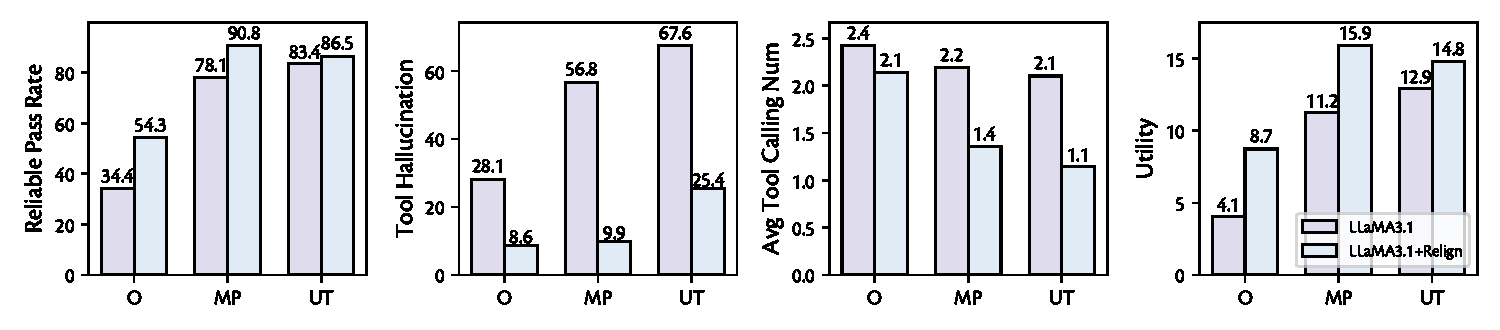
\includegraphics[width=\linewidth]{figs/metrics_grouped.pdf}
    \vspace{-10mm}
    \caption{Comparison of performance metrics between the baseline and Relign across three subsets: Original (O), Missing Parameter (MP), and Unmatched Tools (UT).}
    \label{fig:main_results}
\end{figure*}


\begin{figure}[t!]
    \centering
    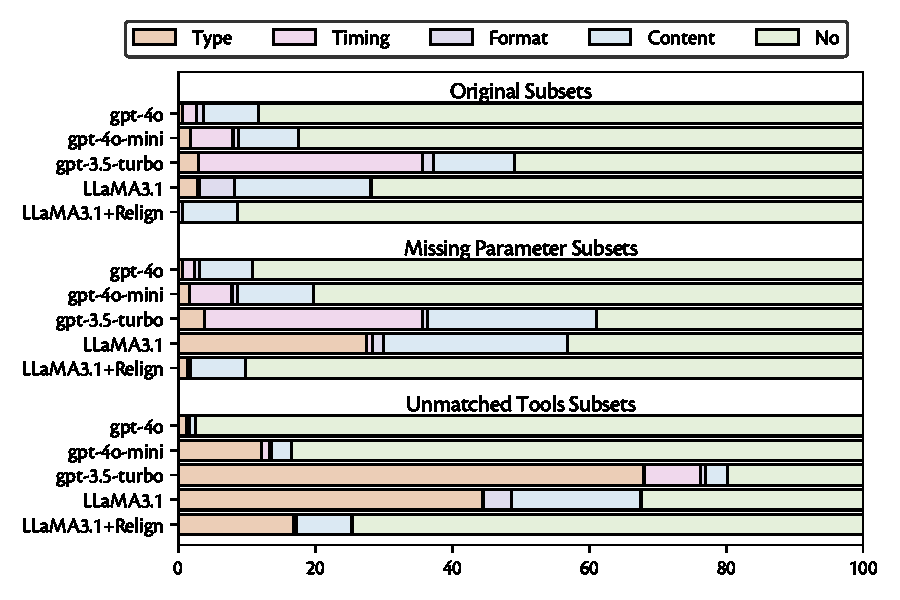
\includegraphics[width=\linewidth,trim=10 10 10 10,clip]{figs/hallu_dist.pdf}
    \vspace{-4mm}
    \caption{\textbf{Distribution of tool hallucination types.} The results highlight the effectiveness of Relign in reducing hallucination across all subsets.}
    \label{fig:hallu_type}
\end{figure}

% \begin{figure}[t!]
%     \centering
% 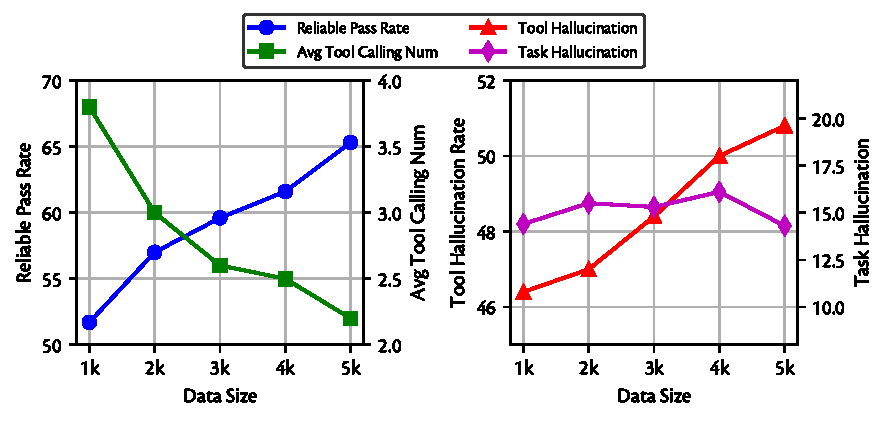
\includegraphics[width=\linewidth,trim=5 5 5 5,clip]{figs/metrics_data_size.pdf}
%     \vspace{-4mm}
%     \caption{\textbf{Comparison of performance metrics between different training data sizes.}}
%     \label{fig:data_size}
% \end{figure}

% \begin{figure}[t!]
%     \centering
% 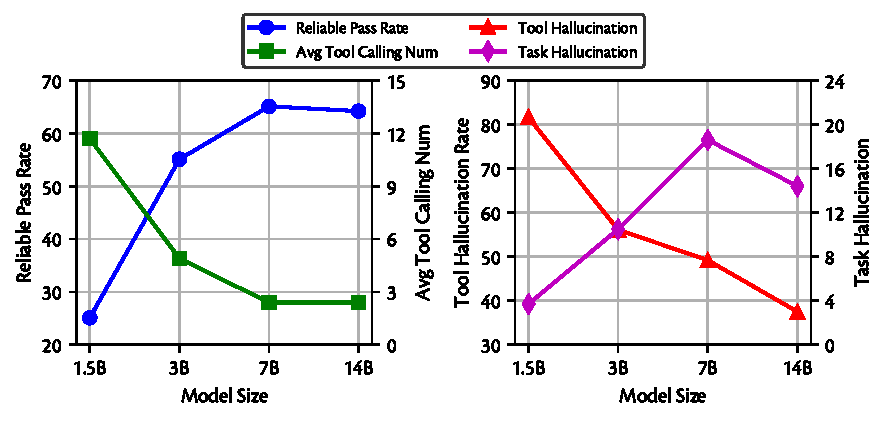
\includegraphics[width=\linewidth,trim=5 5 5 5,clip]{figs/metrics_model_size.pdf}
%     \vspace{-4mm}
%     \caption{\textbf{Comparison of performance metrics between different model sizes.}}
%     \label{fig:model_size}
% \end{figure}

As shown in Table~\ref{table:main_res}, we assessed the performance of our model on three subsets of StableToolbench. Our primary focus was on measuring the tool hallucination rate and the task pass rate. Our results indicate that the implementation of the Reliability Alignment framework, which includes both SFT and DPO, significantly reduces the tool hallucination rate of the baseline model. Moreover, we observed a decrease in the average number of tool callings required for each task. Although previous tool-learning methods, such as StepTool, effectively improve task success rates, they provide no reduction in tool hallucination rates and do not decrease the number of tool calls. In contrast, our approach not only enhances task success rates but also significantly reduces hallucinations. Furthermore, our Relign-trained model based on LLaMA 3.1 outperforms many closed-source models of similar scale, such as GPT-3.5-Turbo and GPT-4o Mini, approaching the performance of GPT-4o.


Figure~\ref{fig:main_results} further demonstrates the effectiveness of our Relign framework in reducing tool hallucination and improving system efficiency across three categories of subsets: Original (O), Missing Parameter (MP), and Unmatched Tools (UT). Relign achieves a remarkable and consistent improvement in all the metrics over all subsets. 
% Our method achieves a remarkable improvement in the Reliable Pass Rate, particularly in the UT subset, where the rate increases from 90.5\% in the baseline to 97.8\%. Similarly, the Tool Hallucination rate experiences a drastic reduction, dropping from 83.0\% to only 4.3\% in the UT subset, highlighting the robustness of our approach in handling mismatched tools. Furthermore, the Average Tool Calling Number decreases significantly across all subsets, with the UT subset seeing a reduction from 4.0 calls in the baseline to just 0.2 calls, showcasing the enhanced ability to reject unmatched tool usage. Finally, our framework maximizes task Utility, with the UT subset showing a substantial increase from 13.8 in the baseline to 19.2, underscoring the practical benefits of our alignment strategies in achieving both reliable and resource-efficient task execution.


% \subsection{Reliability Evaluation}

% Table 2 presents the comprehensive results of the reliability evaluation across different models and methods. In this table, we focus on two key metrics: \textbf{Utility} and \textbf{Ratio}. From the data, it is evident that our proposed approach significantly improves both the utility and ratio compared to the baseline models. Although the combination of SFT and DPO slightly reduces the task pass rate, the substantial reduction in tool hallucinations and unnecessary tool callings leads to a marked increase in both utility and ratio. This improvement indicates better system reliability, as the model becomes more efficient in task completion with fewer errors related to tool usage. The higher utility and ratio values demonstrate that our alignment method not only reduces hallucinations but also enhances the system’s effectiveness in reliably handling complex tasks. 

% \input{tables/hallucination_type.tex}

\subsection{Tool Hallucination Analysis}
Figure~\ref{fig:hallu_type} provides a detailed distribution of different types of tool hallucinations. With Relign framework, all hallucination types show significant reductions, with the greatest improvement observed in the Content Hallucination category, particularly in the Unmatched Tools subset. However, Timing Hallucination demonstrates a relatively smaller improvement, likely due to the inherent difficulty in learning the sequential dependencies required to avoid repetitive or redundant tool calls. This underscores the robustness of our method while identifying areas for further optimization.

% Specifically, within the I1 instruction subset, the predominant hallucinations are tool timing hallucination and tool content hallucination. In the Missing Parameter subset, Tool Content Hallucination is the most common type of error, while in the Unmatched Tools subset, tool type Hallucination dominates. Experimental results demonstrate that our alignment framework enables the model to learn how to accurately assess both the purpose and correct usage of tools, significantly reducing hallucinations in tool selection and usage, and thereby improving the overall reliability of tool callings. Across all subsets, the method demonstrates a consistent reduction in the occurrence of various types of hallucinations. Notably, in the Unmatched Tool subset, our model successfully eliminates hallucinations entirely, bringing the hallucination rate to zero. This significant improvement enhances the reliability of tool usage across the entire subset and reduces hallucination-related errors, ultimately contributing to more accurate and dependable tool interactions.

\subsection{Comparison with Existing Metrics}
Our RePR metric is a refined version of Pass Rate, as we found that some tasks in the original pass rate metric exhibited result hallucinations. Therefore, we believe the pass rate has certain inaccuracies and did not include its results in our paper. As shown in the Table~\ref{table:existing_metrics}, we have supplemented some of the original Pass Rate results. The results indicate that RePR is lower than Pass Rate, and the gap is more pronounced in base models without Relign alignment. This suggests that unaligned models tend to produce more tool hallucinations, which in turn mislead the final results. Moreover, whether using Pass Rate or RePR, our Relign framework consistently improves task success rates.

\begin{table}[!ht]
\centering
\setlength\tabcolsep{3pt}
\resizebox{\columnwidth}{!}{%
\begin{tabular}{lcccccccc}
\toprule
\multirow{2}{*}{\centering Method} & \multicolumn{2}{c}{I1 Instruction} & \multicolumn{2}{c}{I2 Category} & \multicolumn{2}{c}{I3 Instruction} & \multicolumn{2}{c}{Overall} \\
\cmidrule(lr){2-3} \cmidrule(lr){4-5} \cmidrule(lr){6-7} \cmidrule(lr){8-9}
& PR & RePR & PR & RePR & PR & RePR & PR & RePR \\
\midrule
ToolLLaMA         & 76.8 & 64.2 & 77.0 & 64.4 & 72.3 & 58.9 & 75.4 & 62.5 \\
\quad\quad + Relign    & 77.1 & 68.2 & 77.3 & 68.3 & 76.2 & 71.0 & 76.9 & 69.1 \\
\midrule
LLaMA3.1          & 83.0 & 68.5 & 84.8 & 66.1 & 80.1 & 61.3 & 82.6 & 65.3 \\
\quad\quad + Relign    & 87.0 & 80.5 & 89.2 & 75.8 & 86.9 & 75.4 & 87.7 & 77.2 \\
\midrule
Qwen2.5           & 86.3 & 71.5 & 84.3 & 66.2 & 80.6 & 57.7 & 83.7 & 65.1 \\
\quad\quad + Relign    & 87.6 & 77.0 & 87.5 & 69.0 & 85.5 & 72.9 & 86.9 & 73.0 \\
\bottomrule
\end{tabular}%
}
\caption{Comparison of models on original Pass Rate and RePR.}
\label{table:existing_metrics}
\end{table}

\subsection{Out-of-distribution Generalization to APIBench}
As shown in the table below, we also evaluate our method on the out-of-domain test set APIBench. We follow the evaluation setup described in ~\citep{qin2023toolllm} (for more details, please refer to ~\citealp{qin2023toolllm}). Rather than training on APIBench, we treat each API in the prompt as a function call to assess how well our trained model generalizes to OOD datasets. Experimental results with two types of tool retrieval indicate that Relign improves model performance on other tool-use tasks as well, suggesting that reducing tool hallucinations helps models learn better tool-use strategies (AST represents tool-calling accuracy).
\begin{table}[!ht]
\centering
\setlength\tabcolsep{3pt}
\resizebox{\columnwidth}{!}{
\begin{tabular}{lcccccc}
\toprule
\multirow{2}{*}{\centering Method} & \multicolumn{2}{c}{HuggingFace} & \multicolumn{2}{c}{TorchHub} & \multicolumn{2}{c}{Tensorhub} \\
\cmidrule(lr){2-3} \cmidrule(lr){4-5} \cmidrule(lr){6-7}
& Hallu.($\downarrow$) & AST($\uparrow$) & Hallu.($\downarrow$) & AST($\uparrow$) & Hallu.($\downarrow$) & AST($\uparrow$) \\
\midrule
LLaMA3.1 + BM25          & 9.7 & 14.3 & 11.7 & 47.8 & 10.5 & 40.3 \\
\quad + Relign + BM25    & \textbf{6.4} & \textbf{15.7} & \textbf{7.9}  & \textbf{50.1} & \textbf{5.5}  & \textbf{42.5} \\
\midrule
LLaMA3.1 + Oracle        & 9.3 & 87.8 & 10.4 & 86.1 & 7.8  & 89.6 \\
\quad + Relign + Oracle  & \textbf{6.5} & \textbf{89.5} & \textbf{7.7}  & \textbf{88.9} & \textbf{3.2}  & \textbf{91.3} \\
\bottomrule
\end{tabular}
}
\caption{OOD generalization experiments on APIBench.}
\label{table:apibench}
\end{table}


\subsection{Discussion}

\begin{figure}[t!]
    \centering
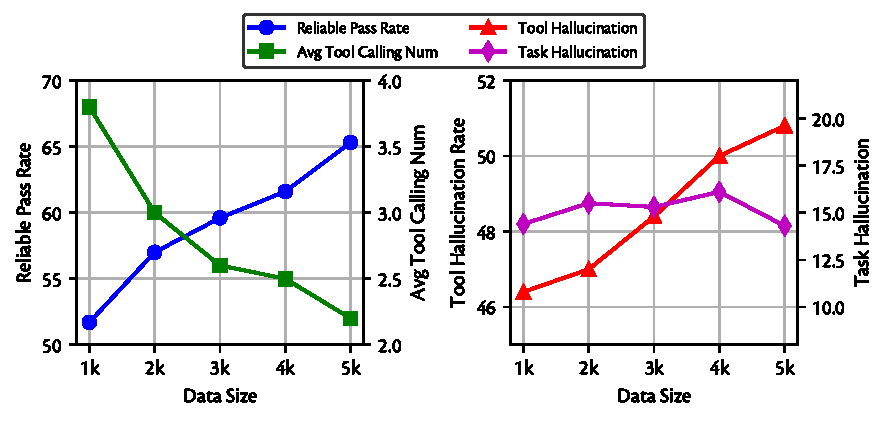
\includegraphics[width=\linewidth,trim=5 5 5 5,clip]{figs/metrics_data_size.pdf}
    \vspace{-4mm}
    \caption{\textbf{Impact of Training Data Size on Performance and Hallucination Metrics.} Experiments are conducted on LLaMA3.1.}
    \vspace{-4mm}
    \label{fig:data_size}
\end{figure}

\paragraph{Does More Data Reduce Hallucination?}
Increasing the amount of training data from 1k to 5k consistently improves model performance, as reflected by the rising Reliable Pass Rate in Figure~\ref{fig:data_size}. However, this increase in data size does not always lead to a reduction in hallucination rates. Both Tool and Task Hallucination rates remain stable or even slightly increase with more data. This could be attributed to overfitting on ToolBench data, which consists of well-structured tool interaction trajectories and lacks samples that handle edge cases (e.g., failure scenarios where a task cannot be completed). Thus, the model learns correct tool calls but struggles with failure scenarios, defaulting to excessive hallucinated tool calls instead of invoking indecisive actions—precisely the issue Relign aims to address.

\begin{figure}[t!]
    \centering
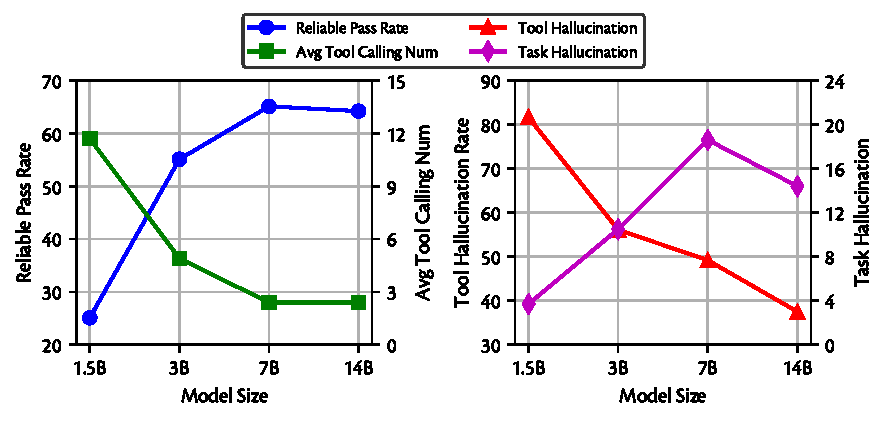
\includegraphics[width=\linewidth,trim=5 5 5 5,clip]{figs/metrics_model_size.pdf}
    \vspace{-4mm}
    \caption{\textbf{Impact of Model Size on Performance and Hallucination Metrics.} Experiments are conducted on Qwen2.5 with 5k data.}
    \vspace{-4mm}
    \label{fig:model_size}
\end{figure}

\paragraph{Does a Larger Model Reduce Hallucination?}
Scaling up model size from 1.5B to 14B, while keeping the training data fixed at 5k, leads to significant improvements in both performance and hallucination reduction, as seen in Figure~\ref{fig:model_size}. Larger models exhibit a better ability to capture complex task dependencies and context, resulting in a noticeable decline in both tool hallucinations and excessive tool calls, leading to more reliable and efficient tool use. Moreover, the Reliable Pass Rate increases with model size, highlighting the enhanced robustness and generalization capabilities of larger models. These results suggest that scaling model parameters is a key strategy for improving the reliability and accuracy of tool usage in complex environments.

